\chapter{系统架构}

本文提出一个基于可编程网卡的高性能数据中心系统架构。
如图 \ref{arch:fig:virt-architecture} 所示,网卡是服务器与外界通信的 ``网关'',也可以作为服务器内硬件设备、虚拟机间通信的 ``枢纽''。
我们把普通网卡升级为可编程网卡,将虚拟化、网络和存储功能、操作系统中需要高性能的数据平面卸载到可编程网卡,以降低 ``数据中心税'',让 CPU 集中精力于客户的应用程序。


\begin{figure}[htbp]
	\centering
	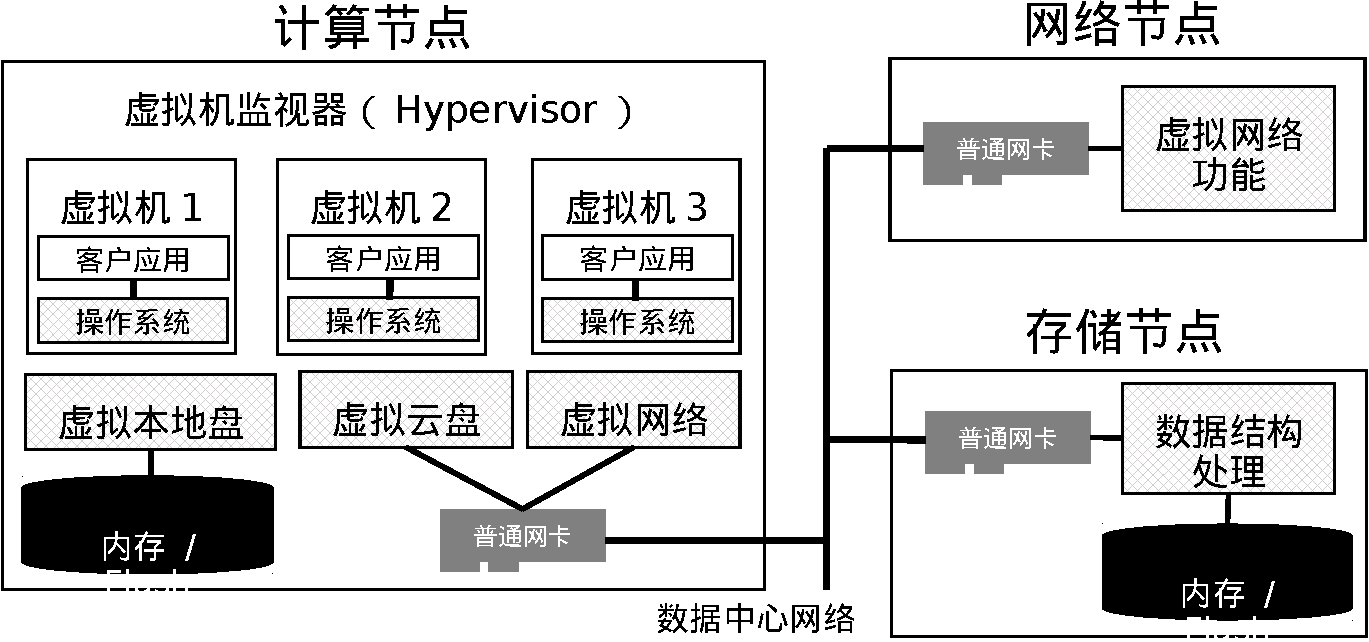
\includegraphics[width=0.8\textwidth]{figures/virt_arch.pdf}
	\caption{回顾:虚拟化的数据中心架构。}
	\label{arch:fig:virt-architecture}
\end{figure}

第 \ref{chapter:intro} 章已经讨论过,虚拟化的数据中心主要可以分为计算、网络、存储节点。
在网络和存储节点,我们采用控制面与数据面分离的设计思想。数据面是操作相对频繁、逻辑相对简单的处理,而控制面是操作相对不频繁、逻辑相对复杂的处理。我们在可编程网卡中实现数据面,在主机 CPU 上实现控制面,实现了数据面完全不经过主机 CPU。这包括第 \ref{chapter:clicknp} 章的虚拟网络功能和第 \ref{chapter:kvdirect} 章的数据结构处理。加速虚拟网络功能和远程数据结构访问也是本文最重要的创新。

在计算节点,亦即客户虚拟机所在的服务器主机上,我们用可编程网卡实现虚拟机监控器(hypervior)的虚拟化功能和操作系统原语。
虚拟化分为 ``一虚多'' 和 ``多虚一'' 两个方面。
``一虚多'',即可编程网卡把计算节点内的硬件资源虚拟化成多个逻辑资源,实现其他计算节点和本地多台虚拟机的多路复用。例如,第 \ref{chapter:clicknp} 章的 ClickNP 将硬件网卡和网络链路虚拟化为每个虚拟机一张虚拟网卡;第 \ref{chapter:clicknp} 章的 KV-Direct 实现了多个客户端并发访问共享键值存储,并能保证一致性。
``多虚一'',即可编程网卡把数据中心内物理上分散的资源虚拟化成一个逻辑资源,实现逻辑资源到物理资源的映射和路由。例如,第 \ref{chapter:clicknp} 章的 ClickNP 将数据中心内网络功能虚拟化成逻辑上统一的网络功能;第 \ref{chapter:clicknp} 章的 KV-Direct 客户端将分布式键值存储虚拟化成逻辑上统一的键值映射;还可以实现存储和内存的解聚(disaggregation)。
为了加速操作系统原语并控制硬件的复杂度,我们把操作系统原语划分为可编程网卡上的可靠通信协议和主机 CPU 上运行的用户态库、用户态管理程序,如第 \ref{chapter:socksdirect} 章 SocksDirect 实现的套接字通信原语。

图 \ref{arch:fig:accel-arch} 显示了基于可编程网卡的系统总体架构。下面我们将按照网络、存储和高层抽象的顺序,简要介绍本文后续各章的总体设计。


\begin{figure}[htbp]
	\centering
	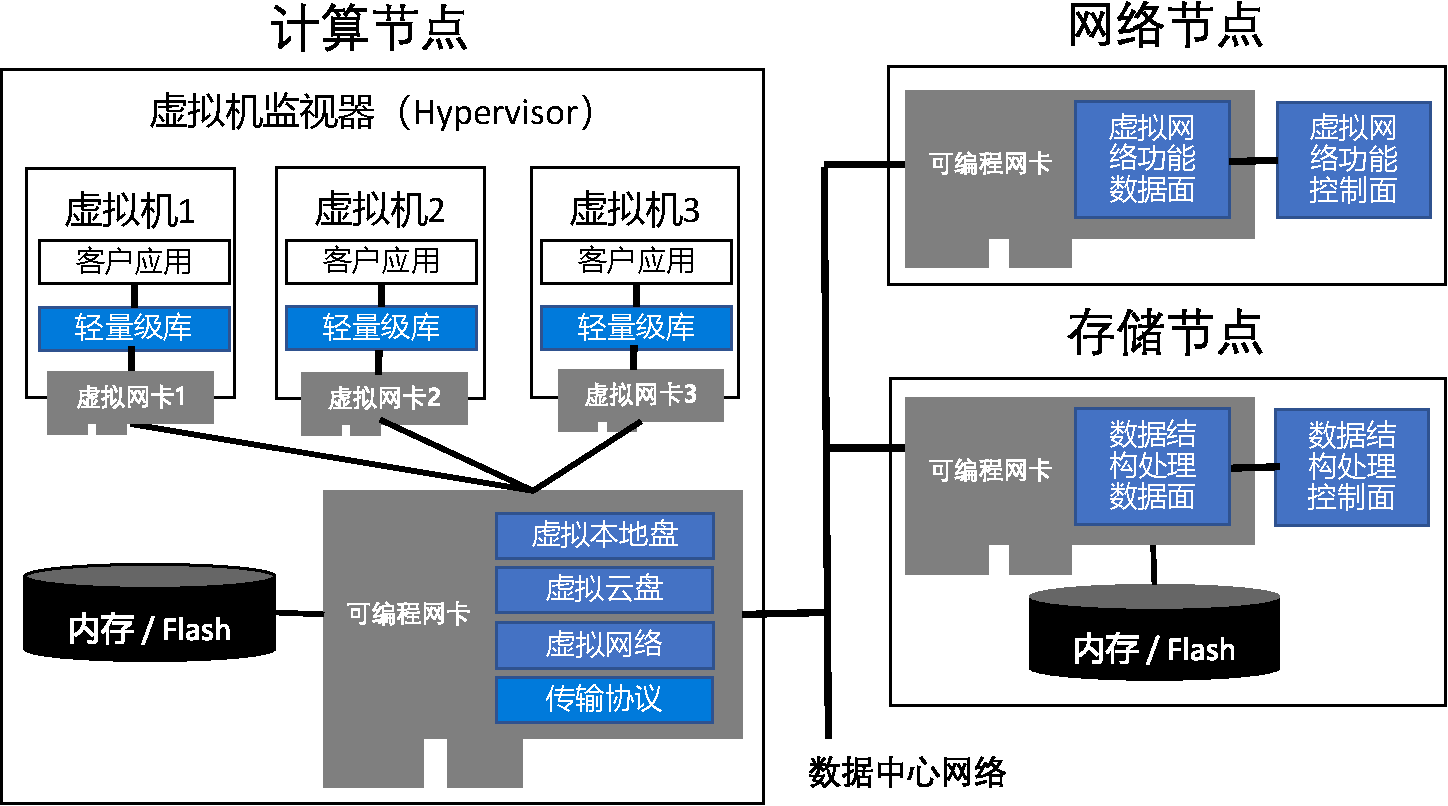
\includegraphics[width=0.8\textwidth]{figures/accel_arch.pdf}
	\caption{基于可编程网卡的数据中心系统总体架构。}
	\label{arch:fig:accel-arch}
\end{figure}



\section{网络加速}

\subsection{网络虚拟化加速}

我们从第 \ref{chapter:intro} 章的传统数据中心架构(图 \ref{intro:fig:virt-architecture})开始,逐步把 ``数据中心税'' 消除或者卸载(offload)到可编程网卡上。
如图 \ref{arch:fig:virtual-network} 所示,第一步是用可编程网卡替代原有的普通网卡,并把软件实现的虚拟网络卸载到可编程网卡上。

\begin{figure}[htbp]
	\centering
	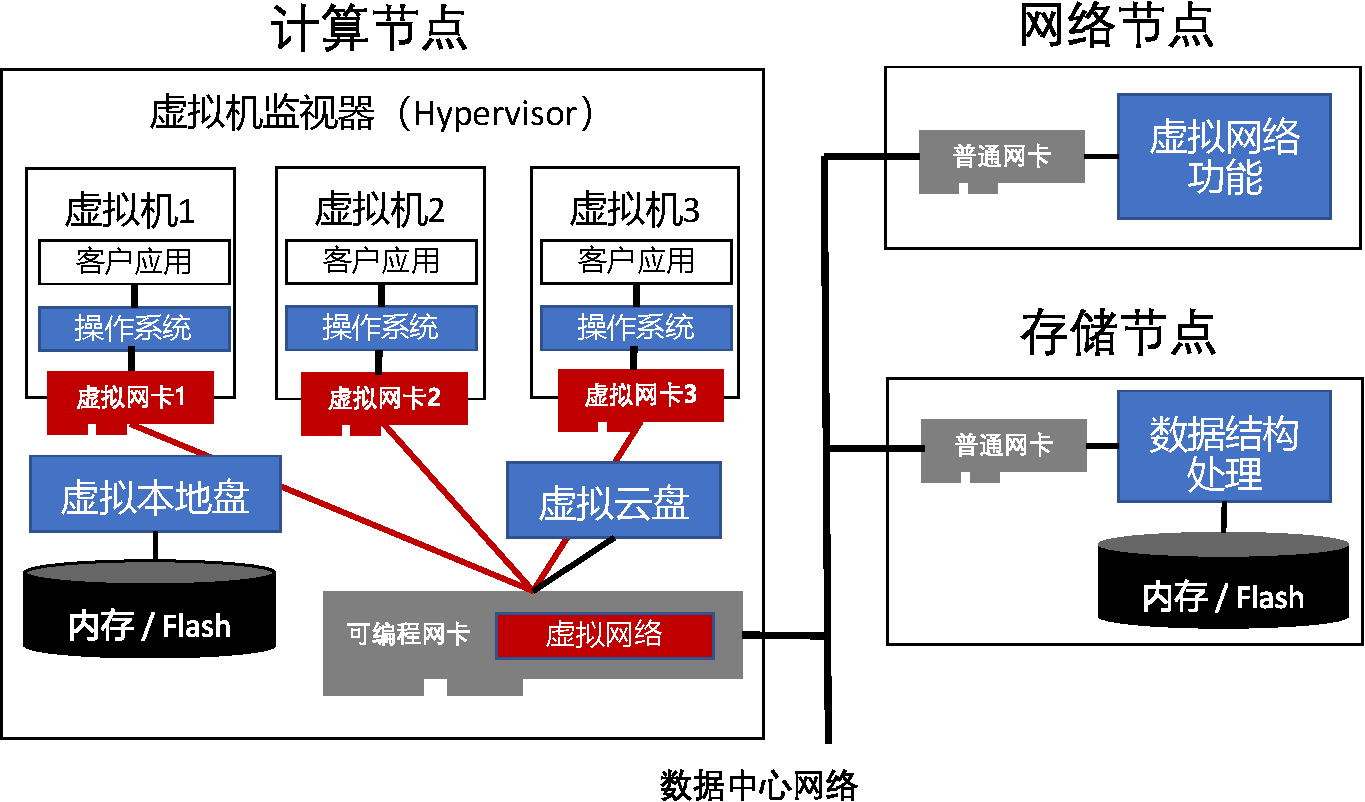
\includegraphics[width=0.8\textwidth]{figures/virtual_network.pdf}
	\caption{用可编程网卡加速虚拟网络后的架构。}
	\label{arch:fig:virtual-network}
\end{figure}


为了让虚拟机上的操作系统网络协议栈能够使用虚拟网络收发数据包,可编程网卡利用 SR-IOV(Single Root I/O Virtualization)技术 \cite{dong2012high},虚拟化成多个 PCIe 虚拟设备(VF,Virtual Function),并给每台虚拟机分配一个 PCIe 虚拟设备。
虚拟机内原有的虚拟网卡驱动程序(如基于 virtio 技术 \cite{russell2008virtio} 的)需要替换为本文实现的 FPGA 驱动程序和基于 FPGA 的虚拟网卡驱动程序。
第 \ref{chapter:clicknp} 章的 ClickNP 将硬件网卡和网络链路虚拟化为多个租户的虚拟网络。

如果我们可以绕过虚拟机操作系统的网络协议栈,直接替换虚拟机上应用程序所使用的标准库(即系统调用接口 libc),就不必实现 SR-IOV 硬件虚拟化。
第 \ref{chapter:socksdirect} 章的 SocksDirect 通过截获应用程序关于网络套接字的标准库调用,在用户态实现了容器覆盖网络(container overlay network),即适用于容器的虚拟网络。
为了用户态运行库与可编程网卡间的高效通信,我们在虚拟机内安装 FPGA 驱动程序,将可编程网卡的 PCIe 地址空间的一部分映射到用户态,从而绕过了虚拟机内核和虚拟机监视器(Virtual Machine Monitor 或 Hypervisor)。



\subsection{网络功能加速}

如图 \ref{arch:fig:network-function} 所示,第二步是在网络节点上,把软件实现的虚拟网络功能划分为数据面和用户面,并把数据面卸载到可编程网卡中。
需要注意的是,网络节点和计算节点的划分是逻辑上的。有可能虚拟网络功能被编排到与虚拟机相同的服务器主机上,这时网络节点和计算节点的功能就合二为一了,虚拟网络和虚拟网络功能之间的连接也从数据中心网络简化成了可编程网卡内模块间的连接。

来自源计算节点(或上一个网络节点)的数据包被网络节点的可编程网卡接收之后,在网卡内的数据面进行处理,大多数情况下不需要 CPU 上的控制面介入,就可以把处理后的数据包再发送回数据中心网络,到达目的计算节点(或下一个网络节点)。
第 \ref{chapter:clicknp} 章将介绍如何用高级语言模块化编程实现网络功能,实现 FPGA 数据面与 CPU 控制面的协同处理。


\begin{figure}[htbp]
	\centering
	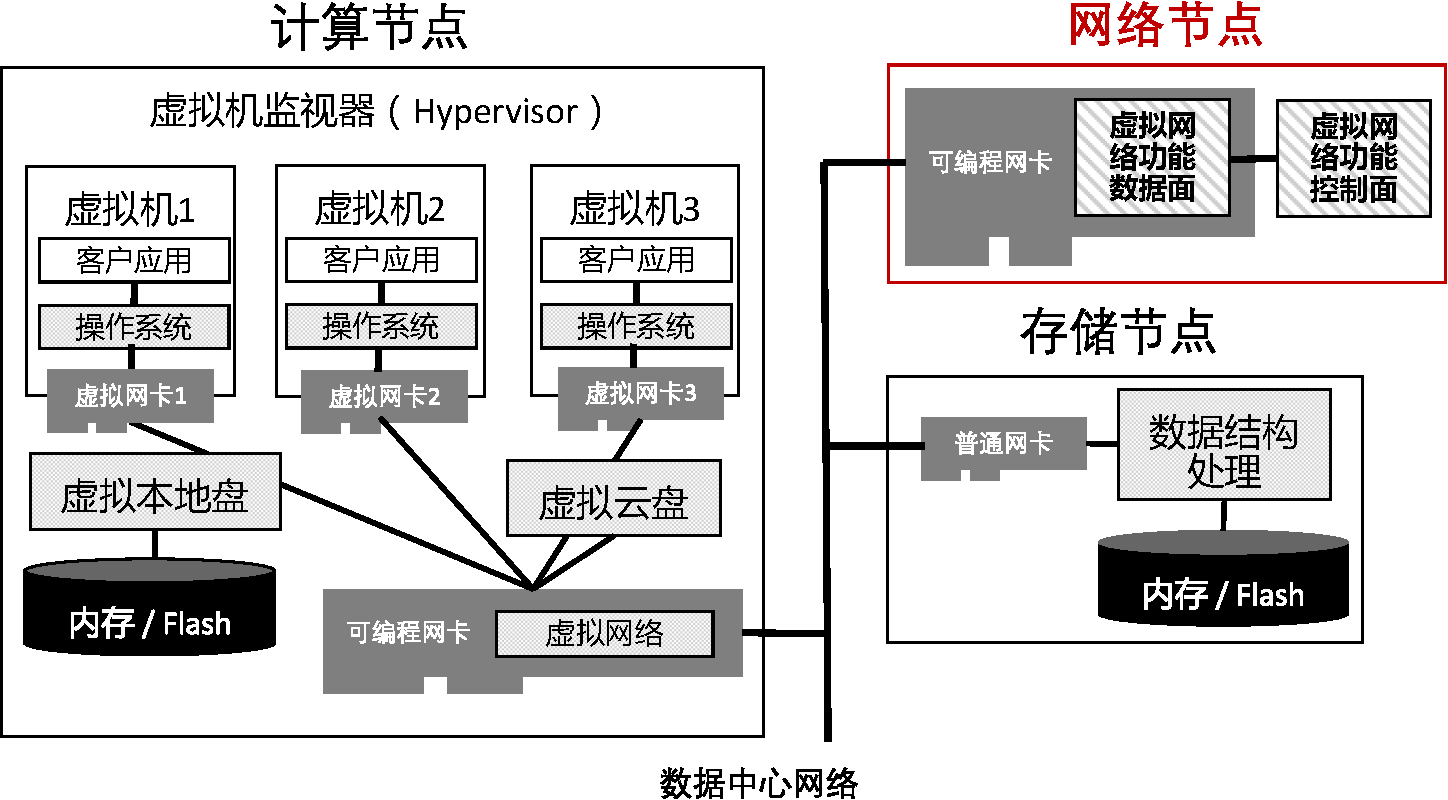
\includegraphics[width=0.8\textwidth]{figures/NFV_accel.pdf}
	\caption{用可编程网卡加速网络功能后的架构。}
	\label{arch:fig:network-function}
\end{figure}

\section{存储加速}

\subsection{存储虚拟化加速}

在网络加速之后,第三、四步是存储加速。作为第三步,我们首先计算节点的存储虚拟化功能卸载到可编程网卡中。
虚拟机需要两种访问块存储(block storage)的方式:一是通过操作系统的存储协议栈来访问块设备,二是通过用户态的快速接口绕过操作系统直接访问。
由于操作系统本身和很多软件运行在块存储上,保持第一种传统访问方式的兼容性是必要的。
存储性能敏感的应用则使用本文提供的库来通过第二种方式访问块存储。

如图 \ref{arch:fig:virt-storage} 所示,可编程网卡将存储硬件的物理请求队列(如 SATA 的 32 个请求槽位和 NVMe 的请求队列)虚拟化成多个逻辑请求队列,并给第一种访问方式和每个需要第二种访问方式的应用分配一条逻辑请求队列。
由于第一种传统方式仅为提供兼容性,为了降低开发难度,本文没有使用 SR-IOV 技术,而是复用了现有虚拟机监视器中的软件虚拟化方案。
为了提供第二种高效访问方式,我们在虚拟机内安装 FPGA 驱动程序,将逻辑请求队列映射到用户态,从而应用程序可以通过我们的库接口直接访问可编程网卡,绕过了操作系统和虚拟机监控器。

为了支持多个存储节点组成的分布式存储,虚拟云存储服务需要把逻辑地址映射到存储节点地址。例如,在第 \ref{chapter:clicknp} 章的分布式键值存储中,客户端需要根据一致性哈希(consistent hashing) \cite{nishtala2013scaling},把键(key)映射到存储节点,再把请求路由到该节点。

\begin{figure}[htbp]
	\centering
	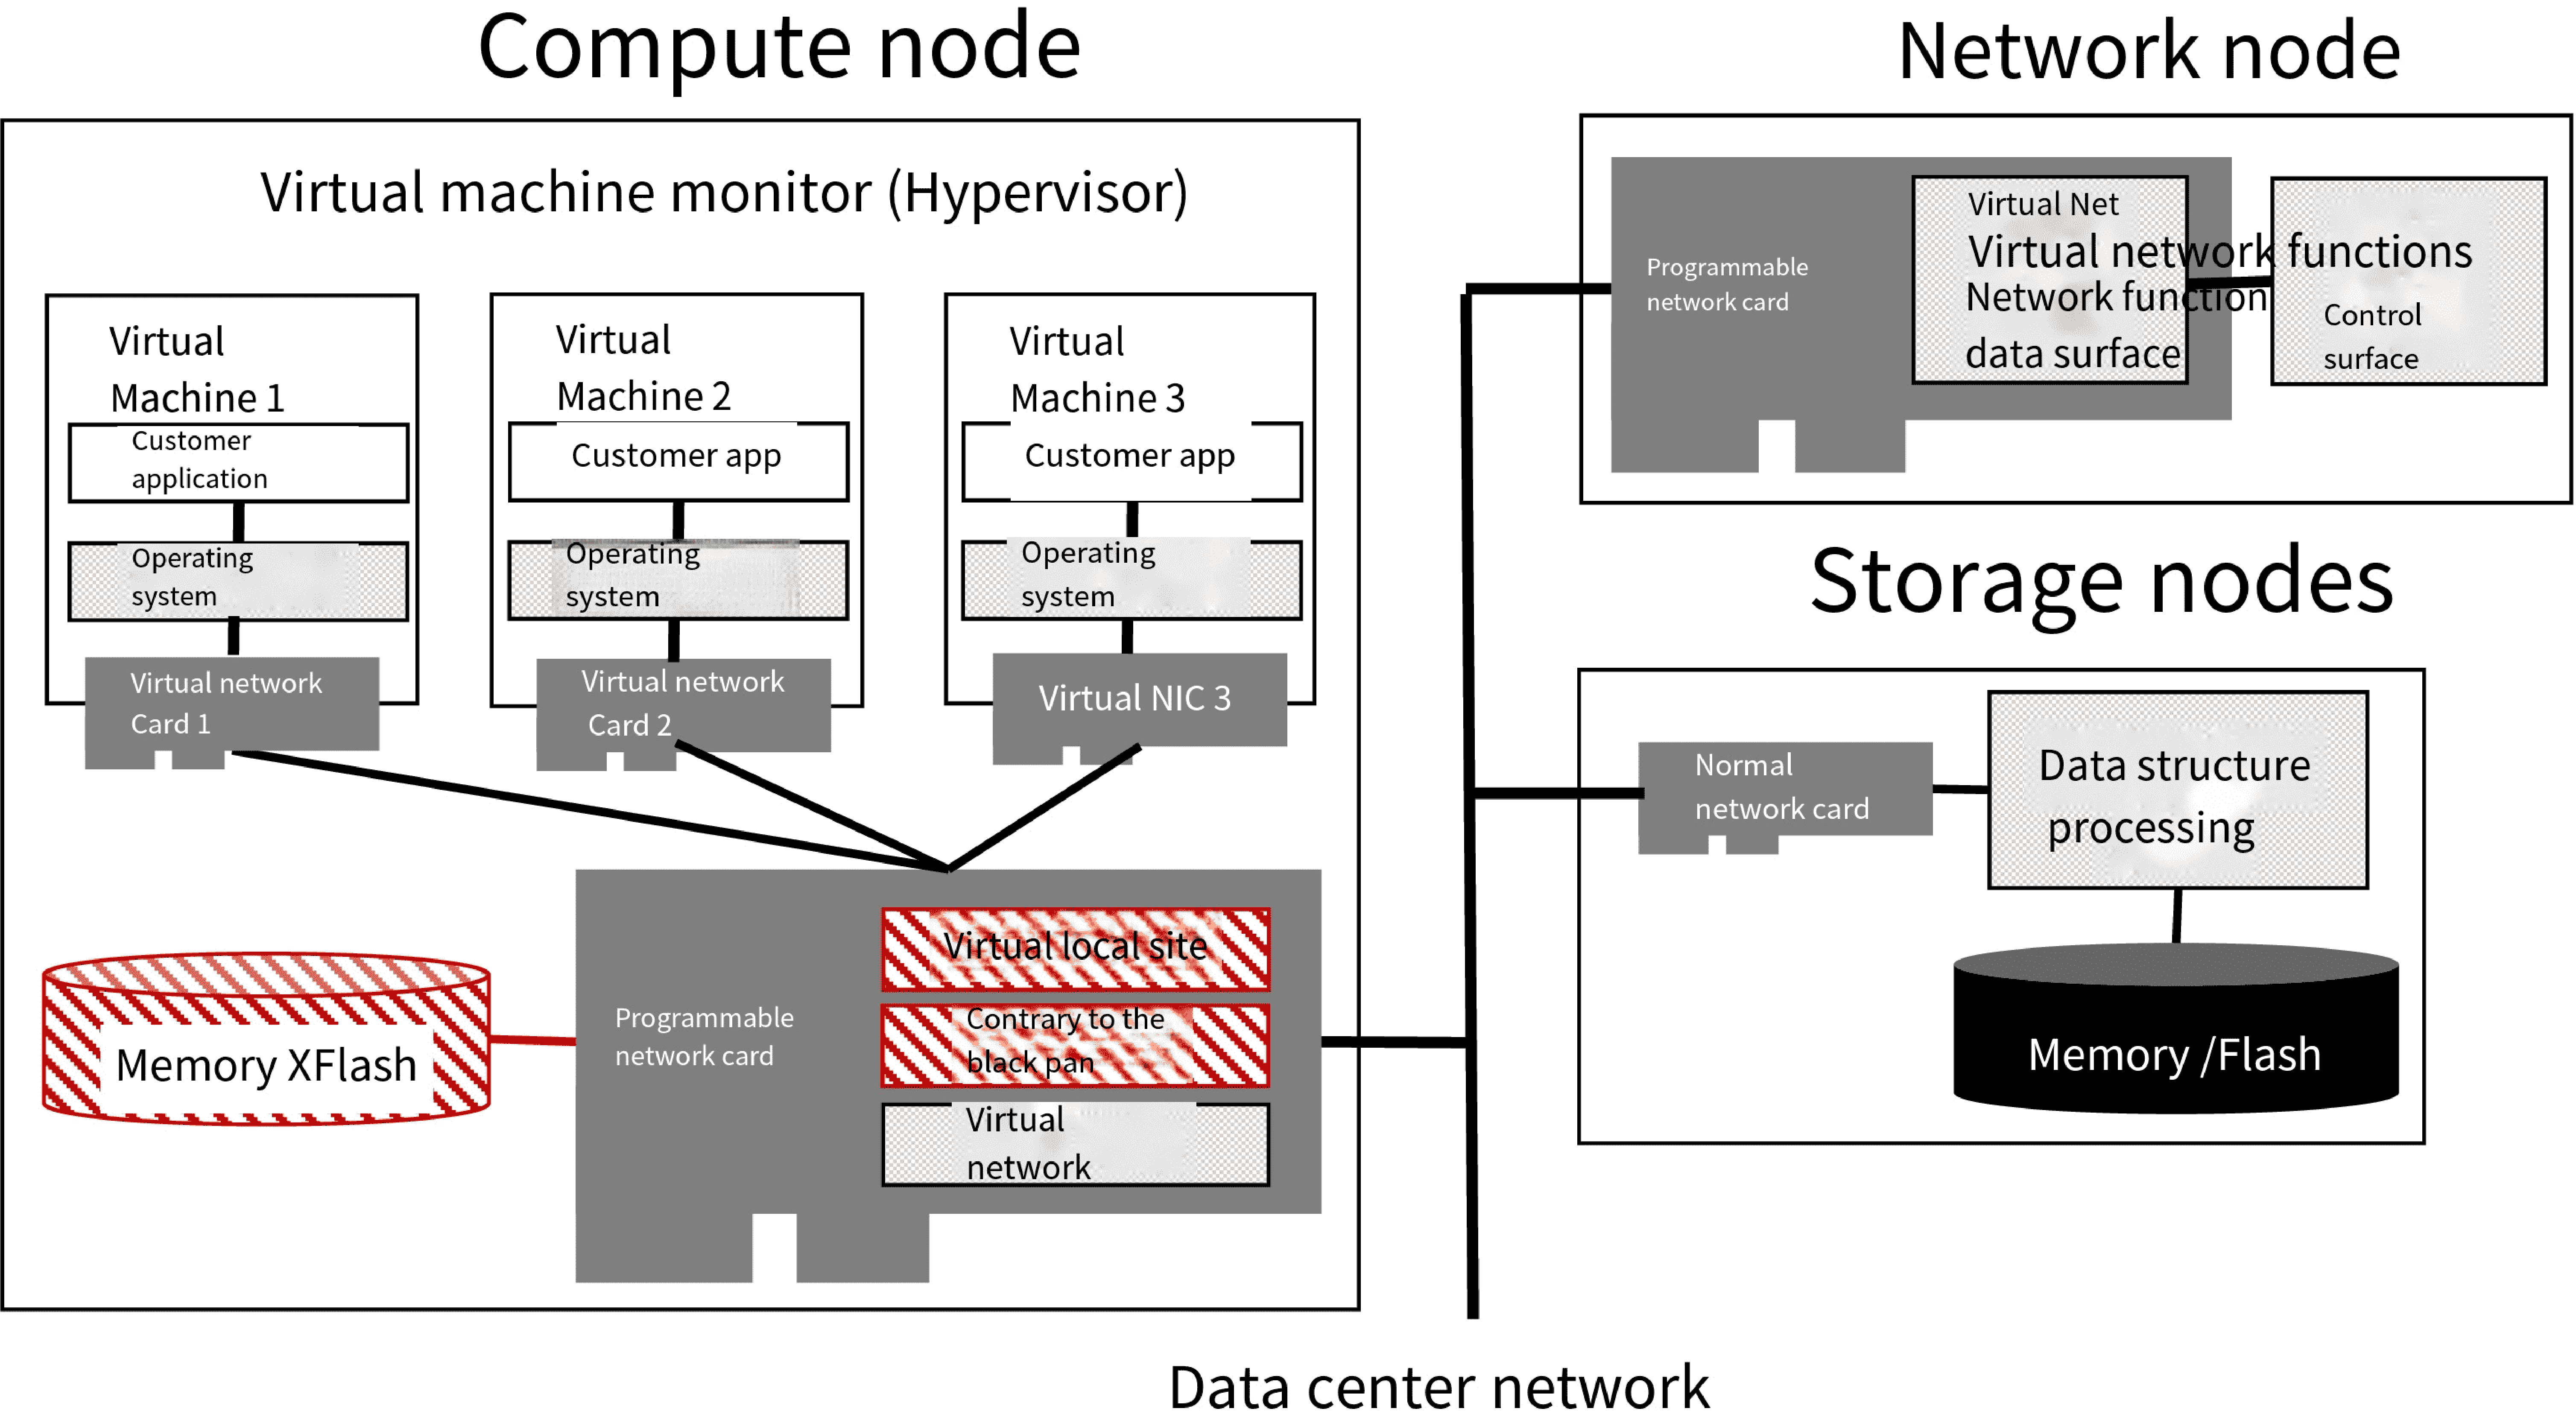
\includegraphics[width=0.8\textwidth]{figures/virt_storage.pdf}
	\caption{用可编程网卡加速本地存储和云存储后的架构。}
	\label{arch:fig:virt-storage}
\end{figure}

\subsection{数据结构处理加速}

第四步,我们将存储节点上的数据结构处理卸载(offload)到可编程网卡。
我们以第 \ref{chapter:kvdirect} 章将详细介绍的键值存储为例。
存储节点上的可编程网卡从网络上收到查询(GET)或写入(PUT)某个键(key)的请求后,要从本地的内存或闪存中查询出对应的键值对,处理请求后把结果发送给网络上的请求方。
如图 \ref{arch:fig:data-structure-accel},这个过程称为数据结构处理的数据面,通常不需要控制面介入。
然而,由于可编程网卡上不适合运行复杂的逻辑,我们把内存分配器分为网卡和主机 CPU 两部分。网卡上缓存若干固定大小的空闲内存块。当空闲内存块不足时,需要主机 CPU 上的控制面通过拆分更大的内存块来补充空闲内存块;当空闲内存块过多时,又需要主机 CPU 来进行垃圾回收,合并成更大的内存块。
通过网卡直接访问内存数据结构的另一个挑战是网卡与内存之间的 PCIe 带宽较低、延迟较高。为此,第 \ref{chapter:kvdirect} 章设计了一系列优化方法来节约带宽、通过并发处理来隐藏延迟。
尽管请求是并发处理的,第 \ref{chapter:kvdirect} 章的设计还能保证多个客户端并发访问的强一致性,即请求在逻辑上按照网络接收的顺序被依次处理。
如果存储节点同时也作为计算节点运行虚拟机,为了解决本地和远程访问同一块存储区域时的一致性问题,不管是本地还是远程访问,都经过可编程网卡处理。

\begin{figure}[htbp]
	\centering
	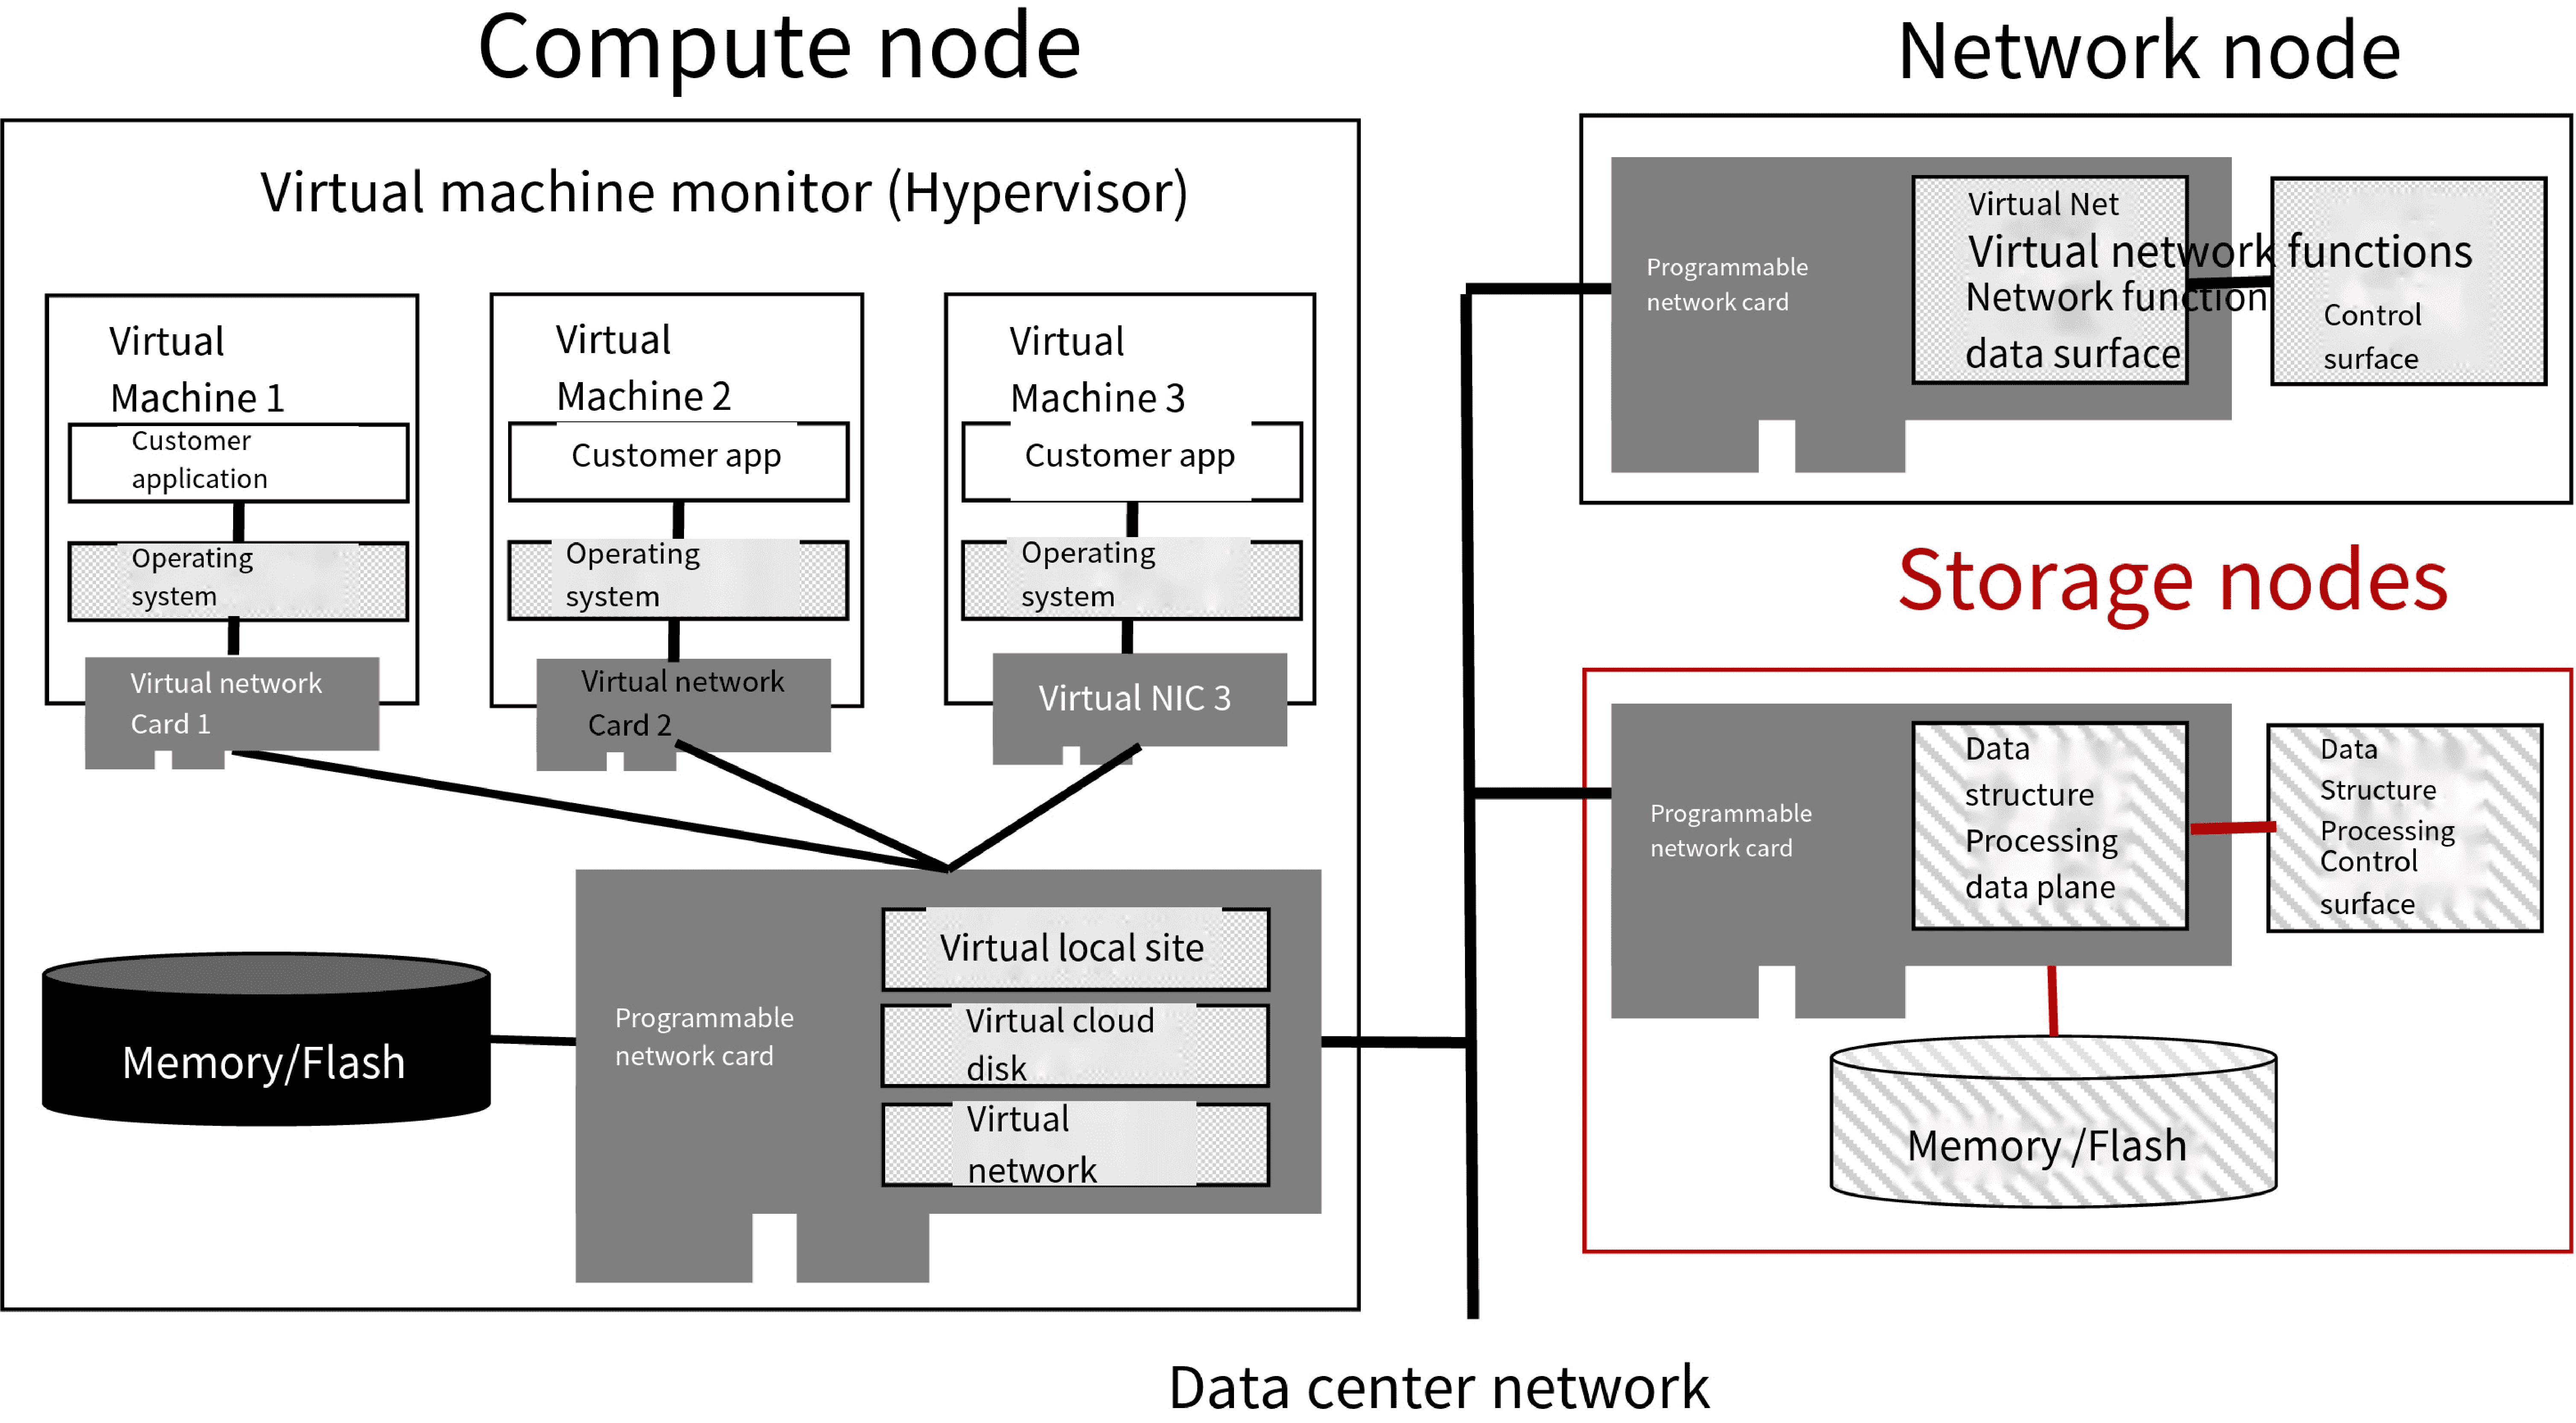
\includegraphics[width=0.8\textwidth]{figures/data_structure_accel.pdf}
	\caption{用可编程网卡加速数据结构处理后的架构。}
	\label{arch:fig:data-structure-accel}
\end{figure}

\section{操作系统加速}

最后一步,我们将操作系统中需要高性能的功能拆分为三部分,分别在可编程网卡、主机 CPU 的用户态运行库和主机 CPU 的用户态守护进程(daemon)中处理。
如图 \ref{arch:fig:os-primitives-accel},操作系统在图中被替换成了用户态运行库,而可编程网卡中增加了传输协议的功能。
用户态运行库通过替换标准库(如 libc),截获了应用程序的系统调用,从而可以在用户态实现操作系统功能的一部分,而把另一部分功能卸载到可编程网卡。
用户态守护进程主要用于控制面操作,为简化起见,图 \ref{arch:fig:os-primitives-accel} 中没有画出。

\begin{figure}[htbp]
	\centering
	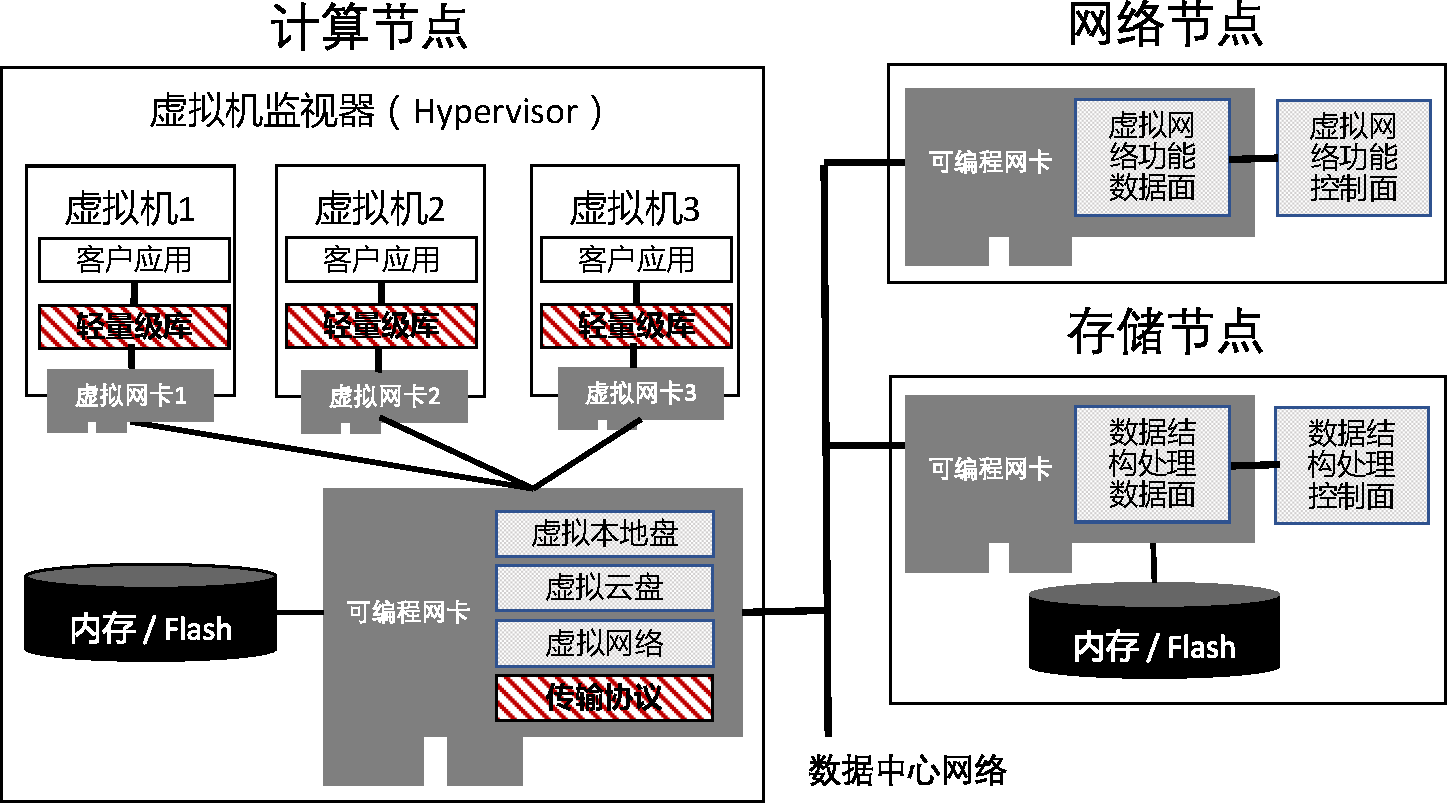
\includegraphics[width=0.8\textwidth]{figures/os_primitives_accel.pdf}
	\caption{用可编程网卡加速操作系统通信原语后的架构。}
	\label{arch:fig:os-primitives-accel}
\end{figure}

操作系统中包括通信、存储等子系统,本文以通信系统的加速为例。套接字是应用程序最常用的通信原语,但由于操作系统的多种开销,其性能不令人满意。
第 \ref{chapter:socksdirect} 章设计并实现了一个高性能的用户态套接字系统,与现有应用程序完全兼容,并且对主机内进程间通信和跨主机的通信都能达到接近硬件极限的低延迟和高吞吐量。
系统由可编程网卡上的可靠通信协议和主机 CPU 上运行的用户态库、用户态守护进程三部分构成。
对于跨主机的通信,数据面由可编程网卡和用户态库构成,可编程网卡负责多路复用和可靠传输等低层语义,提供远程直接内存访问(RDMA)原语;用户态库负责把 RDMA 原语封装成 Linux 虚拟文件系统(Virtual File System)的套接字语义,提供无锁消息队列、缓冲区管理、等待事件、零拷贝内存页面重映射等高层语义。
对于主机内的通信,数据面由 CPU 的硬件内存一致性协议(coherence protocol)和用户态库构成。用户态库在进程间建立共享内存队列,并依靠 CPU 的内存一致性协议自动同步。用户态库的功能与跨主机通信类似。
用户态守护进程负责控制面,即初始化、进程创建和退出、连接建立和关闭、与 RDMA 网卡建立队列、在进程之间建立共享内存队列等。

在第 \ref{chapter:socksdirect} 章的设计中,客户应用程序通过 SocksDirect 运行库,直接访问可编程网卡中的 RDMA 功能,不需要经过操作系统内核和虚拟机监控器,可编程网卡也就不需要支持 SR-IOV 硬件虚拟化。



\section{可编程网卡}

在结束基于可编程网卡的数据中心系统架构介绍后,本节介绍可编程网卡内部的软硬件架构。如图 \ref{arch:fig:sw-hw-codesign} 所示,可编程网卡内的逻辑主要由第 \ref{chapter:clicknp} 章的编程框架、第 \ref{chapter:kvdirect} 章的基础服务中间件以及第 \ref{chapter:kvdirect} 章和第 \ref{chapter:socksdirect} 章的应用层构成。主机 CPU 上配套的软件包括第 \ref{chapter:clicknp} 章的 FPGA 通信库和驱动程序、第 \ref{chapter:kvdirect} 章的键值操作库和第 \ref{chapter:socksdirect} 章兼容 Linux 操作系统的套接字通信库。

\begin{figure}[htbp]
	\centering
	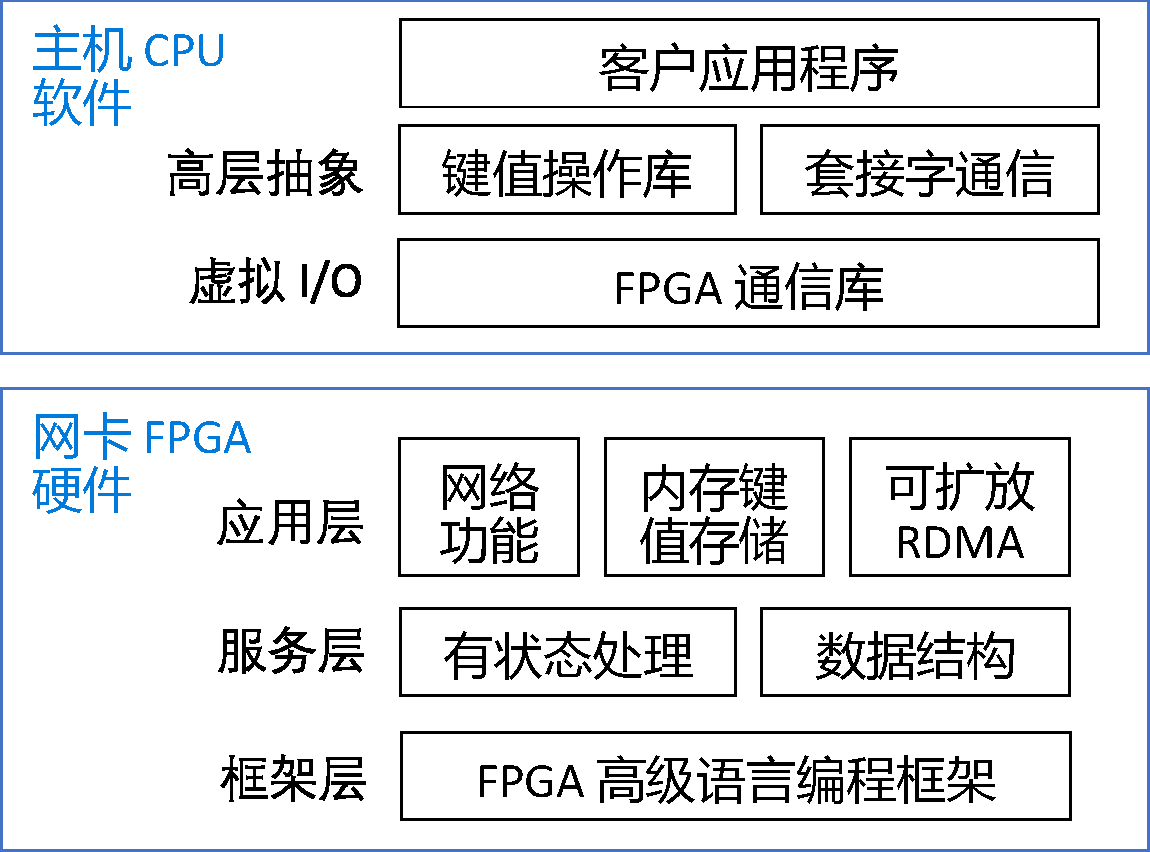
\includegraphics[width=0.5\textwidth]{figures/sw_hw_codesign.pdf}
	\caption{软硬件协同设计的可编程网卡架构。}
	\label{arch:fig:sw-hw-codesign}
\end{figure}


\subsection{硬件架构}


图 \ref{arch:fig:smartnic-current} 显示了本文使用的 Catapult 可编程网卡 \cite{putnam2014reconfigurable} 硬件架构。
本文第 \ref{chapter:clicknp} 章和第 \ref{chapter:kvdirect} 章使用其中的 FPGA 可重构逻辑来实现网络功能和数据结构处理;第 \ref{chapter:socksdirect} 章使用其中的商用 RDMA 网卡实现套接字原语中的硬件传输协议部分。
来自数据中心网络的数据包从 FPGA 左上角的网络接口被可编程网卡接收。如果它是网络功能或者数据结构处理需求,就直接在 FPGA 可重构逻辑中进行处理,处理过程中 FPGA 需要使用板上 DRAM 和通过 CPU 互连(如 PCIe)访问主机 DRAM。
如果数据包是用于第 \ref{chapter:socksdirect} 章中的套接字通信,它将在 FPGA 中进行虚拟网络的解封装,并通过 FPGA 与商用 RDMA 网卡之间的网络接口发送给商用 RDMA 网卡。
商用 RDMA 网卡会把数据包的内容通过 CPU 互连(如 PCIe) DMA 发送给主机上的用户态套接字库。

\begin{figure}[htbp]
	\centering
	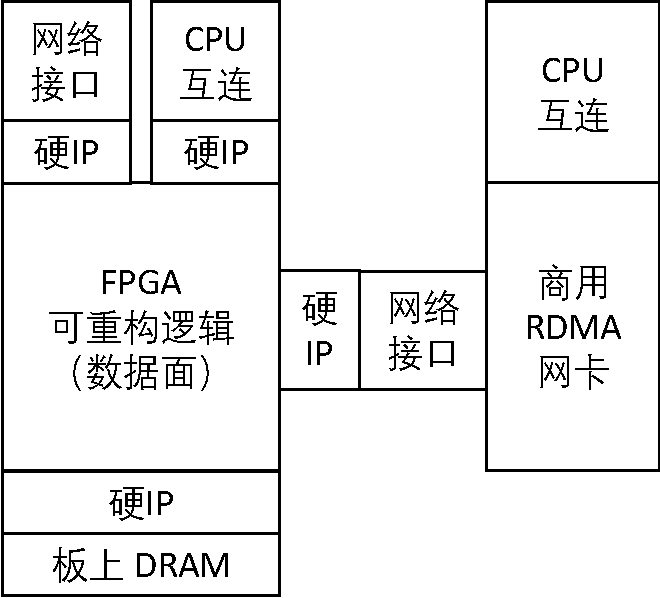
\includegraphics[width=0.4\textwidth]{figures/smartnic-current.pdf}
	\label{arch:fig:smartnic-current}
	\caption{本文使用的 Catapult 可编程网卡。}
\end{figure}







\subsection{高级语言编程框架}

第 \ref{chapter:clicknp} 章将提出适合流式处理的模块化 FPGA 高级语言编程框架 ClickNP。
如图 \ref{arch:fig:element_arch} 所示,ClickNP 的基本处理模块是元件(element)。元件之间使用管道(channel)连接。
每个元件使用类 C 语言编程,可以被编译成 FPGA 上的逻辑模块或者 CPU 上的线程。
每个元件逻辑上可以类比成一个 CPU 核,是一个状态机,由私有内部状态、全局状态、若干输入管道、若干输出管道、数据处理函数和信号处理函数构成。
全局状态使用板上 DRAM 实现,私有内部状态使用片上 BRAM 或寄存器实现。
FPGA 上逻辑模块之间的管道用先进先出队列(FIFO)实现,CPU 上线程之间的管道用共享内存队列实现,FPGA 和 CPU 元件之间的管道用 PCIe I/O 管道实现。
数据处理函数从输入管道中读取数据,处理后发送到输出管道中。信号处理函数用于响应主机控制程序的信号。

\begin{figure}[htbp]
	\centering
	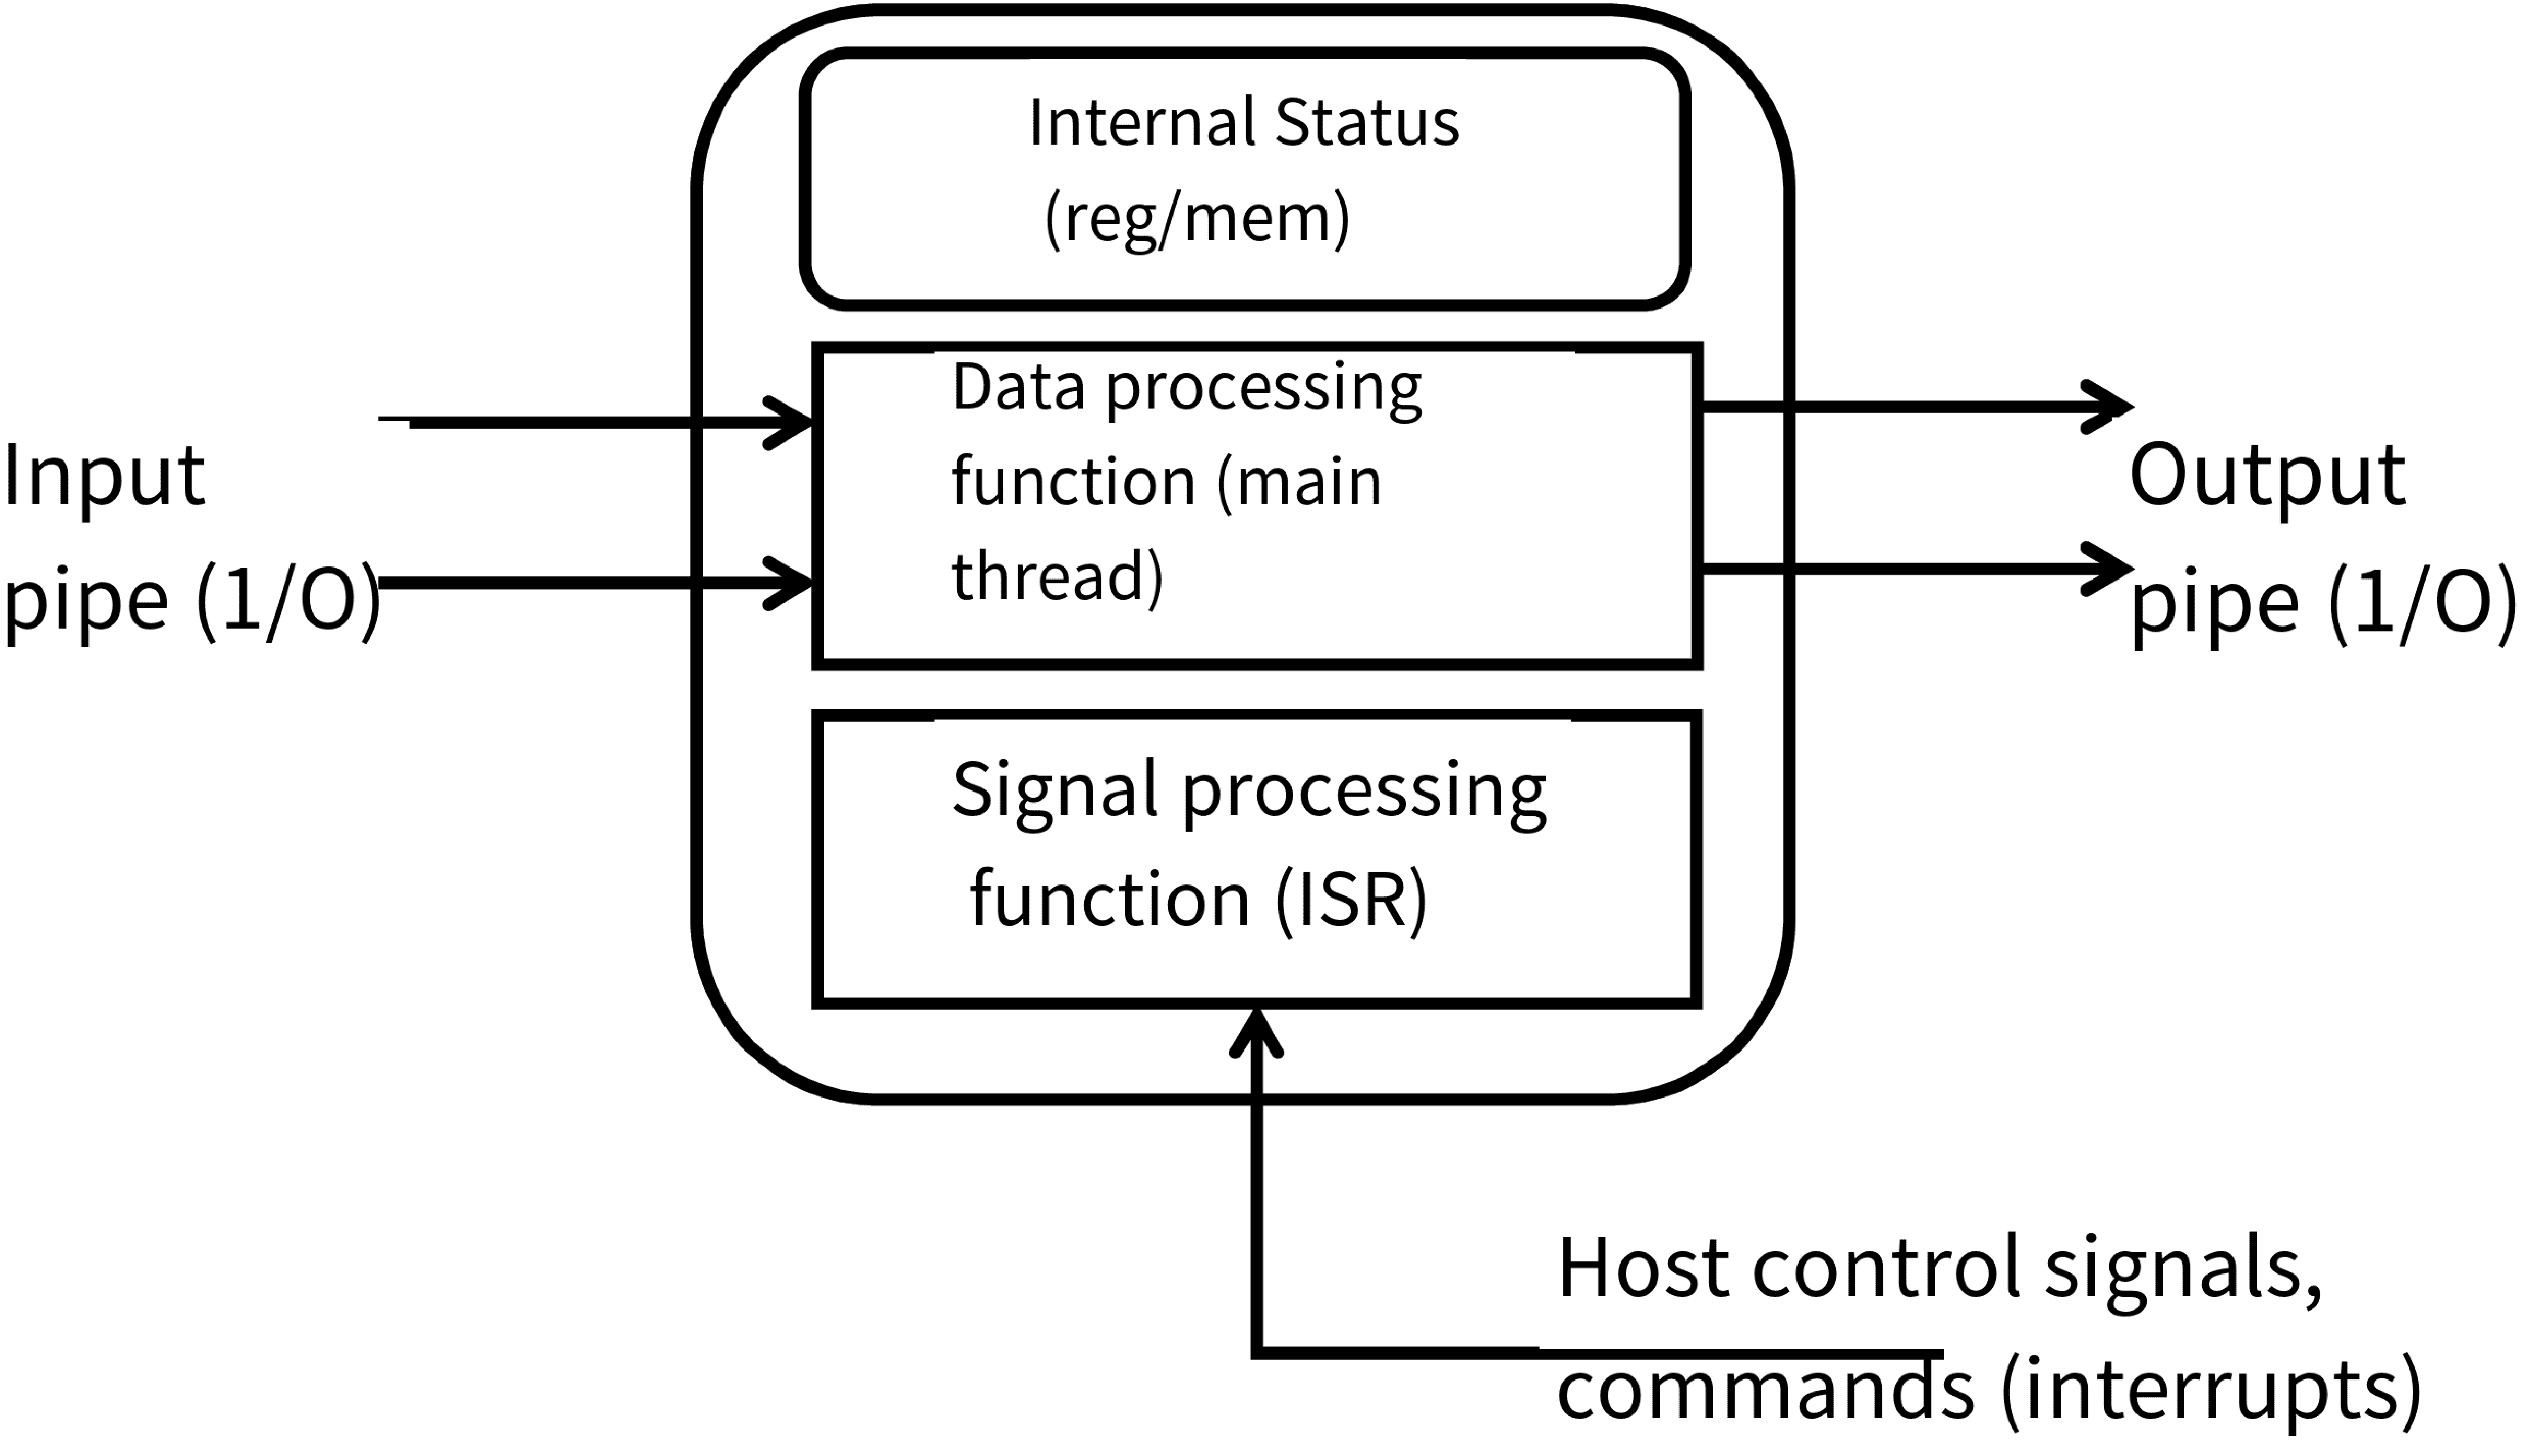
\includegraphics[width=0.5\textwidth]{chapters/clicknp/image/element_arch.pdf}
	\caption{ClickNP 编程框架中的元件。}
	\label{arch:fig:element_arch}
\end{figure}

元件的结构设计使其能实现无阻塞、完全流水线的数据处理。
元件不仅可以在主机上用传统软件开发工具进行调试和测试,ClickNP 编程框架还可以为其生成调试逻辑,实现在 FPGA 运行过程中的日志、断点、查询状态等调试功能。
此外,在虚拟机热迁移(live migration)和高可用(high availability,HA)中,网卡等外设中的状态备份和迁移是一个挑战。
ClickNP 编程框架可以自动生成状态导入导出逻辑,并与管道输入输出控制配合,可以通过状态迁移实现元件和虚拟机的热迁移,通过热备份或冷备份实现可编程网卡不同等级的高可用性。

\subsection{基础服务中间件}

第 \ref{chapter:clicknp} 章的 ClickNP 架构比较适合无状态或状态简单的流水线式数据包处理,而对基于连接状态或应用层请求的处理,就显得捉襟见肘。
例如,第 \ref{chapter:clicknp} 章四层负载均衡器应用中的调度器和哈希表与应用逻辑耦合紧密,既不容易扩放到大量并发连接,代码的可维护性也不强,事实上在开发过程中花费了大量的时间来解决死锁问题。
第 \ref{chapter:kvdirect} 章的 KV-Direct 系统将提出 FPGA 内的有状态处理(stateful processing)和哈希表数据结构设计,这些基础组件是第 \ref{chapter:clicknp} 章的有状态网络功能、第 \ref{chapter:kvdirect} 章的内存键值存储、第 \ref{chapter:socksdirect} 章的可扩放 RDMA 的基础。

为了模块化和可扩放性,使用 KV-Direct 作为基础后,可编程网卡上应用的架构如图 \ref{arch:fig:kvdirect_arch} 所示。
事务代表着前后依赖关系,例如有状态网络处理中的一个连接,分多个数据包的一个应用层 HTTP 请求,或者键值存储中对同一个键(key)的操作。
同一个事务中的不同请求需要依次处理,而不同事务中的请求可以并发处理。
为了隐藏延迟、最大化并发处理能力,请求调度器从基于 KV-Direct 的事务状态键值存储中查找该请求对应的事务编号,并将正在处理事务的请求排入队列。
基于 ClickNP 的数据处理流水线根据请求数据和事务状态进行处理,在处理过程中可能查询其他的数据结构(如内存分配表、主机虚拟地址映射表、防火墙规则表、路由表等)。
如果请求处理完成,响应数据进入输出重排模块,重新排列响应的顺序以满足事务处理的一致性要求(例如,不同事务的请求也要按照到达顺序依次响应),最终输出到网络。
如果请求的处理还需要依赖下一数据包或从主机内存 DMA 来的数据,为了不阻塞数据处理流水线,该请求会返回到调度器,等待依赖操作完成后再进行下一阶段的处理。


\begin{figure}[htbp]
	\centering
	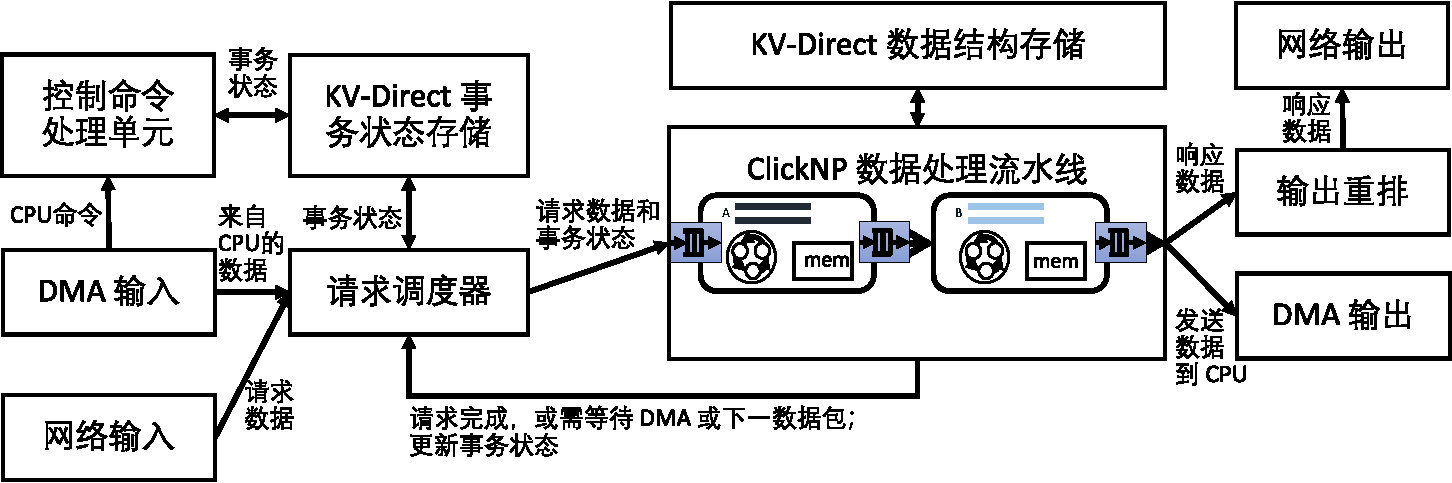
\includegraphics[width=1.0\textwidth]{figures/kvdirect_arch.pdf}
	\caption{基于 KV-Direct 的可编程网卡应用层架构。}
	\label{arch:fig:kvdirect_arch}
\end{figure}

在下面三章中,我们将依次详细讨论本文的三个主要创新点,即基于可编程网卡的网络功能(ClickNP)、存储数据结构(KV-Direct)和操作系统通信原语(SocksDirect)加速。
